%
% b2skal.tex -- Skalierung eines B2 Wavelets
%
% (c) 2019 Prof Dr Andreas Müller, Hochschule Rapperswil
%
\documentclass[tikz]{standalone}
\usepackage{amsmath}
\usepackage{times}
\usepackage{txfonts}
\usepackage{pgfplots}
\usepackage{csvsimple}
\usetikzlibrary{arrows,intersections,math}
\begin{document}
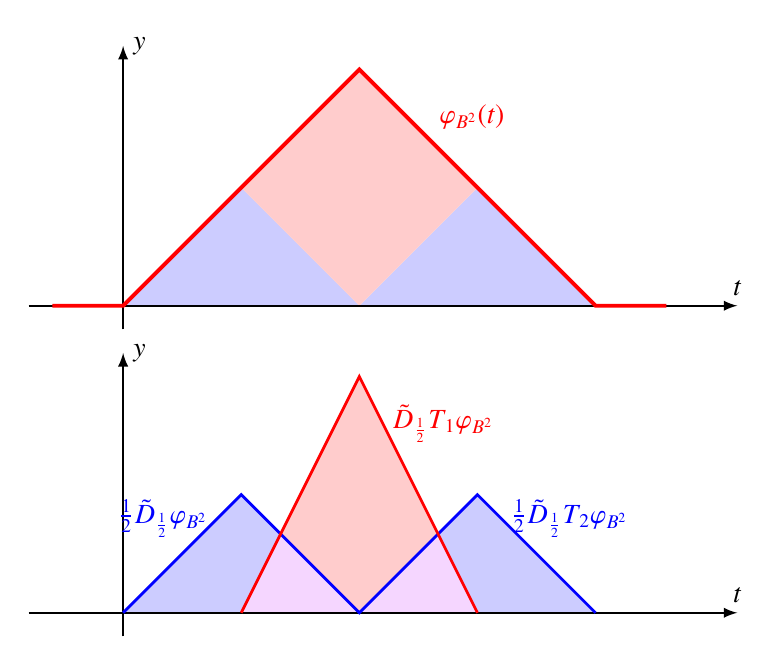
\begin{tikzpicture}[>=latex,scale=3]

\definecolor{pink}{rgb}{0.8,0.2,1}

\fill[color=blue!20] (0,0)--(1,0)--(0.5,0.5)--cycle;
\fill[color=blue!20] (1,0)--(2,0)--(1.5,0.5)--cycle;
\fill[color=red!20] (0.5,0.5)--(1,0)--(1.5,0.5)--(1,1)--cycle;

\draw[->,line width=0.7pt] (-0.4,0)--(2.6,0) coordinate[label={$t$}];
\draw[->,line width=0.7pt] (0,-0.1)--(0,1.1) coordinate[label={right:$y$}];

\draw[line width=1.4pt,color=red]
	(-0.3,0)--(0,0)--(1,1)--(2,0)--(2.3,0);

\node[color=red] at (1.3,0.8) [right] {$\varphi_{B^2}(t)$};

\begin{scope}[yshift=-1.3cm]
\fill[color=red!20] (0.5,0)--(1.5,0)--(1,1)--cycle;
\fill[color=blue!20] (0,0)--(1,0)--(0.5,0.5)--cycle;
\fill[color=blue!20] (1,0)--(2,0)--(1.5,0.5)--cycle;
\fill[color=pink!20] (0.5,0)--(1,0)--(0.6666,0.3333)--cycle;
\fill[color=pink!20] (1,0)--(1.5,0)--(1.3333,0.3333)--cycle;

\draw[->,line width=0.7pt] (-0.4,0)--(2.6,0) coordinate[label={$t$}];
\draw[->,line width=0.7pt] (0,-0.1)--(0,1.1) coordinate[label={right:$y$}];

%\draw[color=blue,line width=1pt] (-0.3,0)--(2.3,0);
\draw[color=blue,line width=1pt] (0,0)--(0.5,0.5)--(1,0)--(1.5,0.5)--(2,0);
\draw[color=red,line width=1pt] (0.5,0)--(1,1)--(1.5,0);

\node[color=blue] at (0.4,0.4) [left] {$\frac12\tilde{D}_{\frac12}\varphi_{B^2}$};
\node[color=blue] at (1.6,0.4) [right] {$\frac12\tilde{D}_{\frac12}T_2\varphi_{B^2}$};
\node[color=red] at (1.1,0.8) [right] {$\tilde{D}_{\frac12}T_1\varphi_{B^2}$};
\end{scope}

\end{tikzpicture}
\end{document}

